\documentclass[8pt,a4paper]{article}
\usepackage[utf8]{inputenc}
\usepackage{spconf}
\usepackage{amsmath}
\usepackage{amsfonts}
\usepackage{amssymb}
\usepackage{lmodern}
\usepackage{graphicx}
\usepackage{float}
\usepackage{multicol}
\usepackage{algorithm}
\usepackage{algorithmic}
\usepackage{url}
\usepackage{ftnright}
\usepackage[xindy]{glossaries}
\usepackage{wrapfig}
\usepackage[left=.75cm,right=.75cm,top=.75cm,bottom=.75cm]{geometry}

\graphicspath{{graphics/}}

\twoauthors
  {R. Deliallisi}
  {
  	ETH Zürich, D-INFK\\
  }
  {C. Trassoudaine\sthanks{Work performed while at ETH Zürich}}
  {
	  IMT Atlantique,\\
	  EURECOM, Data Science dpt.
  }
  
\title{
	Robustness verifier heuritics for neural networks
}

\newacronym{nn}{N.N.}{neural-networks}
\newacronym{lp}{L.-P.}{linear-programming}
\newacronym{ba}{B.A.}{box analysis}

\begin{document}

\maketitle

\section{Problem definition and Analysis techniques}

The purpose of this work is to prove formally the local robustness (from now refered as robustness) with repect to some inputs of \gls{nn} by heuristically combining \gls{ba} and \gls{lp} solving. 
In this paper, we aim to present a time-efficient way of verifying \gls{nn} robustness for large $\epsilon$-perturbations, using the $L_\infty$ norm.

\paragraph*{Box analysis}

A very simple and fast approach to solve the \gls{nn} robustness problem is to use a polyhedra abstract domain and to propagate it across the layers.

\paragraph*{Linear programming}

A more precise but more computationaly intensive technique to verify the robustness of a \gls{nn} is to use a linear solver to propagate the box while approximating better the non-linearities. This can be used of two ways: compute the boxes for a given layer using modeling constraints and the previous layers box values, or directly check for robustness on the last layers based on the previous computed boxes.

We here generaly prefer using \gls{lp} on the first layers of the \gls{nn} not to propagate growing boxes. An analogy can be drawn with low-noise amplifiers in the physics field, for which it is really important to keep the noise minimal at the beginning of the process.

\section{Heuristics}

In this section we will refer to Box Analysis as ELINA and Linear Programmming range propagation as GUROBI within the algorithm sections as these are the used tools in our implementation.

\paragraph*{Greedy approach}

The first approach and most efficient one for small \gls{nn}s is to iterate over the layers and using \gls{nn} at each step and verifiyng with \gls{ba} as an exit condition. This takes advantage of the cheap computational cost of \gls{ba} and of the incremental precision of \gls{lp}, which has a cost. The biggest verifiable perturbations will take more time than the smaller ones due to the greater number of \gls{lp} calls, but this also returns results very fast for small perturbations.

\begin{algorithm}[H]
	\scriptsize
	\begin{algorithmic}
		\STATE $n = size(NN)$
		\FOR{$i \in [0, n]$}
		\STATE GUROBI\_OPTIMIZE($Layer_{i+1}$)
		\IF {$Layer_{i+1}$ is the last layer}
		\RETURN {VERIFY($Layer_{n}$)}
		\ELSE
		\STATE ELINA\_RANGE($Layer_{i+1, ..., n}$)
		\IF {VERIFY($Layer_{n}$)}
		\RETURN {\TRUE}
		\ENDIF
		\ENDIF
		\ENDFOR
	\end{algorithmic}
	\caption{Greedy precise algorithm with an early stopping condition}
\end{algorithm}

\paragraph*{Large networks strategy}

The strategy developped for large neural networks is inspired for gradient descent and aims to focus the most on the neurons that propagates the greatest part of the interval length to the last layer neurons that prevent us from verifying the robustness property.

\begin{algorithm}[H]
	\scriptsize
	\begin{algorithmic}
		\STATE $n = size(NN)$
		\STATE{/* \textbf{Compute boxes using ELINA.} */}
		\STATE ($Range_1, ..., Range_n$) = ELINA\_RANGE($Layer_{1, ..., n}$)

		\IF {VERIFY($Layer_{n}$)}
			\RETURN {\TRUE}
		\ELSE
			\STATE{/* \textbf{Backpropagate last layers ranges for which the intersection with true label is not null.} */}
			\STATE $b_1$ = Backpropagate($Range_n$) 

			\STATE{/* \textbf{Optimize most weighted neurons on the first layer based on backpropagation values.} */}
			\STATE $opt_{neurons}$ = index($b_1$, threshold) 
			\STATE $Range_{1,opt_{neurons}}$ = GUROBI\_OPTIMIZE($Layer_{1,opt_{neurons}}$)

			\STATE{/* \textbf{Compute remaining boxes using ELINA.} */}
			\STATE ($Range_2, ..., Range_n$) = ELINA\_RANGE($Layer_{2, ..., n}$)
			\RETURN {VERIFY($Layer_{n}$)}
		\ENDIF
	\end{algorithmic}
	\caption{Large networks heuristic}
\end{algorithm}

Here is a more graphical version:

\begin{figure}[H]
\begin{center}
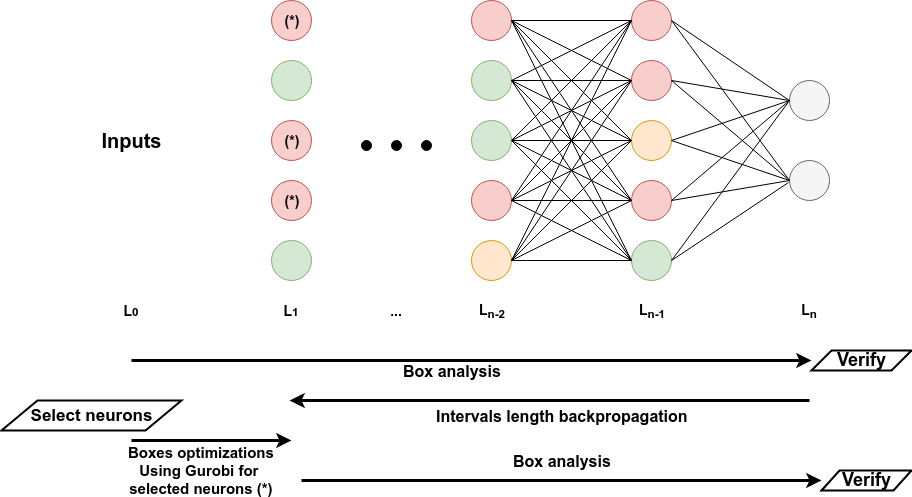
\includegraphics[width=9cm]{NN_lastlayer.png}
\caption{Large networks strategy}
\end{center}
\end{figure}

\section{Performances}

The most important factors in the \gls{lp} analysis complexity seems to be the number of neurons per layer as well as the magnitude of the perturbation. Experimentally, we determined that the complexity for a given network to certify is in $o(exp(\epsilon))$. 
\begin{wrapfigure}{r}{0.23\textwidth}
	\vspace{-30pt}
	\begin{center}
		\small
		\begin{tabular}{| c || l | }
			Layers & neurons per layers \\
			\hline
			3 & 10, 20, 50 \\
			4 & 1024 \\
			6 & 20, 30, 100, 200 \\
			9 & 100, 200 \\
		\end{tabular}
	\end{center}
	\vspace{-11pt}
	\caption{Tested configurations}
	\vspace{-10pt}
\end{wrapfigure}
Hence, reducing the range for the first layers by using \gls{lp} also help to reduce the computational time.

The model performs the analysis in a few minutes for all of the networks and $\epsilon$-perturbations ranging from $10^{-2}$ to $10^{-4}$ using the greedy algorithm for deep-\gls{nn}s and the Large-net strategy for the narrow-\gls{nn}s.

\vfill
\hrule
\end{document}